\documentclass{tex/sig-alternate} 

\newcommand{\TITLE}{Accessing Multiple  Clouds with Cloudmesh}
\newcommand{\AUTHOR}{Gregor von Laszewski} 

%%%%%%%%%%%%%%%%%%%%%%%%%%%%%%%%%%%%%%%%%%%%%%%%%%%%%%%%%%%%%%
% LATEX DEFINITIONS 
%%%%%%%%%%%%%%%%%%%%%%%%%%%%%%%%%%%%%%%%%%%%%%%%%%%%%%%%%%%%%%

\usepackage{textcomp}
\usepackage{mathabx}
\usepackage{enumerate}
\usepackage{hyperref} 
\usepackage{array} 
\usepackage{graphicx} 
\usepackage{booktabs} 
\usepackage{pifont} 
\usepackage{todonotes} 
\usepackage{rotating} 
\usepackage{color} 
\usepackage{tabularx} 
\usepackage{amssymb}
 
\newcommand*\rot{\rotatebox{90}} 
 
\newcommand{\FILE}[1]{\todo[color=green!40]{#1}} 
 
%%%%%%%%%%%%%%%%%%%%%%%%%%%%%%%%%%%%%%%%%%%%%%%%%%%%%%%%%%%%%%
% HYPERSETUP 
%%%%%%%%%%%%%%%%%%%%%%%%%%%%%%`%%%%%%%%%%%%%%%%%%%%%%%%%%%%%%%%

\hypersetup{ 
    bookmarks=true,         % show bookmarks bar 
    unicode=false,          % non-Latin characters in AcrobatΓÇÖs bookmarks 
    pdftoolbar=true,        % show AcrobatΓÇÖs toolbar 
    pdfmenubar=true,        % show AcrobatΓÇÖs menu 
    pdffitwindow=false,     % window fit to page when opened 
    pdfstartview={FitH},    % fits the width of the page to the window 
    pdftitle={\TITLE},    % title 
    pdfauthor={\AUTHOR},     % author 
    pdfsubject={Subject},   % subject of the document 
    pdfcreator={\AUTHOR},   % creator of the document 
    pdfproducer={\AUTHOR}, % producer of the document 
    pdfkeywords={hindex} {cloud}{FutureGrid}, % list of keywords 
    pdfnewwindow=true,      % links in new window 
    colorlinks=false,       % false: boxed links; true: colored links 
    linkcolor=red,          % color of internal links (change box color with linkbordercolor) 
    citecolor=green,        % color of links to bibliography 
    filecolor=magenta,      % color of file links 
    urlcolor=cyan           % color of external links 
} 
 
%%%%%%%%%%%%%%%%%%%%%%%%%%%%%%%%%%%%%%%%%%%%%%%%%%%%%%%%%%%%%%%%%%%%%% 
% HYPHENATION
%%%%%%%%%%%%%%%%%%%%%%%%%%%%%%%%%%%%%%%%%%%%%%%%%%%%%%%%%%%%%%%%%%%%%% 

\hyphenation{cloud-mesh}

%%%%%%%%%%%%%%%%%%%%%%%%%%%%%%%%%%%%%%%%%%%%%%%%%%%%%%%%%%%%%%%%%%%%%% 

\begin{document} 
% 
% --- Author Metadata here --- 
\conferenceinfo{TBD}{} 
\CopyrightYear{2014}  
\crdata{X-XXXXX-XX-X/XX/XX}  % Allows default copyright data (0-89791-88-6/97/05) to be over-ridden - IF NEED BE. 
% --- End of Author Metadata --- 
 
\title{\TITLE} 
%\subtitle{[Extended Abstract] 
%\titlenote{A full version of this paper is available as 
%\texttt{www.acm.org/eaddress.htm}}} 
 
\numberofauthors{1}  
\author{ 
\alignauthor 
Gregor von Laszewski,\titlenote{Corresponding Author.} 
Fugang Wang, 
Geoffrey C. Fox, 
Others to be added ...  \\
       \affaddr{Indiana University}\\
       \affaddr{2719 10th Street}\\
       \affaddr{ Bloomington, Indiana, U.S.A.}\\ 
       \email{laszewski@gmail.com} 
} 
\date{13 March 2014} 
 
\toappear{} 
\maketitle 
\begin{abstract} 

  This paper analyses different aspects of managing multiple clouds
  clouds. We present the design of a toolkit design that can
  practically used by users and administrators to manage multicloud
  environments.  It can either be run by individual users or offered
  as a service to a shared user community. We have practically,
  demonstrated its use as part of a FutureGrid service allowing users
  users of FutureGrid to utilize such a service with their
  credentials. Furthermore, we are discussing implications and
  solutions for a unified metrics system assisting the users to find
  and utilize resources appropriate for their applications. Lastly we
  discuss how to move such a multicloud environment forward by
  integrating clouds managed by the community or are offered as public
  clouds. This includes the introduction of a mutual trust agreements
  on user and project baseis. We have developed a number of components
  that support the creation of such a multicloud environment. This
  system is known as cloudmesh and has been used in practice to
  achieve virtual machine management in multiple clouds. An important
  distinguishing factor of cloudmesh is that it also allows the use of
  bare metal provisioning for supporting service providers and
  authorized users, offering services beyond those available by
  typical clouds.

  The paper will be 8 pages long 
 
\end{abstract} 
 
% A category with the (minimum) three required fields 
\category{H.4}{Information Systems Applications}{Miscellaneous} 
%A category including the fourth, optional field follows... 
\category{D.2.8}{Software Engineering}{Metrics}[complexity measures, performance measures] 
 
\terms{Theory} 
 
\keywords{Cloud}
 
%%%%%%%%%%%%%%%%%%%%%%%%%%%%%%%%%%%%%%%%%%%%%%%%%%%%%%%%%%%%%%%%%%%%%% 
% SECTIONS 
%%%%%%%%%%%%%%%%%%%%%%%%%%%%%%%%%%%%%%%%%%%%%%%%%%%%%%%%%%%%%%%%%%%%%% 

%%%%%%%%%%%%%%%%%%%%%%%%%%%%%%%%%%%%%%%%%%%%%%%%%%%%%%%%%%%%%%%%%%%%%%
\section{Introduction}
%%%%%%%%%%%%%%%%%%%%%%%%%%%%%%%%%%%%%%%%%%%%%%%%%%%%%%%%%%%%%%%%%%%%%%

\subsection{FutureGrid}



FutureGrid \cite{las2010gce,las12fg-bookchapter} ``is a project led by
Indiana University and funded by the National Science Foundation (NSF)
to develop a high performance grid test bed that will allow scientists
to collaboratively develop and test innovative approaches to parallel,
grid, and cloud computing. FutureGrid will provide the infrastructure
to researchers that allows them to perform their own computational
experiments using distributed systems. The goal is to make it easier
for scientists to conduct such experiments in a transparent manner.
FutureGrid users will be able to deploy their own hardware and
software configurations on a public/private cloud, and run their
experiments. They will be able to save their configurations and
execute their experiments using the provided tools. The FutureGrid
test bed is composed of a high speed network connecting distributed
clusters of high performance computers. FutureGrid employs
virtualization technology that will allow the test bed to support a
wide range of operating systems.''



FutureGrid contains a number compute resources organized as part of
clusters with different types and size. They are interconnected with up to a 10GB Ethernet among its sites. The sites include Indiana University, University of Chicago, San Diego Supercomputing Center, Texas Advanced Computing Center, and University of Florida.
In total 481 compute servers with 1126 CPUs and 4496 Cores are
offered. In addition it offers also 448 GPU cores. The total RAM is
about 21.5TB. Secondary storage is about 1PB. A more detailed
description of the resources is provided in
\cite{vonLaszewski-bigdata-bookchapter2014}

FutureGrid offers a very rich environment to its users. We distinguish the following categories: Cloud PaaS, IaaS, GridaaS, HPCaaS, TestbedaaS.

FutureGrid provides an advanced framework to manage user and project affiliation and propagates this information to a variety of subsystems constituting the FG service infrastructure. This includes operational services to deal with authentication, authorization and accounting. In particular we have developed a unique metric framework that allows us to create usage reports from our entire Infrastructure as a Service frameworks. Repeatable experiments can be created with a number of tools including Pegasus, Precip and Cloudmesh.Provisioning of services and images can be conducted by RAIN \cite{imagemanagement,fg-1295}. Infrastructure monitoring is enabled via Nagios \cite{nagios}, Ganglia \cite{ganglia}, and Inca \cite{inca} and our own cloud metric system \cite{las08federated-cloud}.
Within the traditional high performance computing services FG offers a traditional MPI/batch queuing system and a virtual large memory system that are beneficial for big data calculations.


One of the main features of FutureGrid is to offer its users a variety
of infrastructure as a service frameworks
\cite{comparisoncloud,las2011virt} including OpenStack, Eucalyptus,
and Nimbus. These frameworks provide Based on our experience
with FutureGrid over the last couple of years, it is advantageous to
offer a mixed operation model. This includes a standard production
cloud that operates on-demand, but also a set of cloud instances that
can be reserved for a particular project. We have conducted this for
several projects in FutureGrid, including those that required
dedicated access to resources as part of big data research such as
classes \cite{fg405,fg368} or research projects with extremely large
virtual machines \cite{fg298}.


\subsection{Federation}

Cloud federation

Account based federation

Administrative federation

\url{http://www.egi.eu/infrastructure/cloud/}


\cite{kurze2011cloudfederation}


\subsection{Definitions}

To define the federated services that we support with our efforts, we will be
using the following definitions throughout the paper.

\begin{description}
   \setlength{\itemsep}{0pt}
   \setlength{\parsep}{0pt}

\item[public-cloud:]  a service provider makes resources available to
  usres over the public Internet. This includes compute, storage, and
  applications. FutureGrid offers to its users a public cloud. 

\item[private-cloud:] access to services may be having additional
  restrictions. Restrictions could include a limited set of authorized
  users to the services offered or  possible restrictions of exposing services on the public
  internet. FutureGrid offers the ability to set up private clouds for
  special projects. Examples include modified OpenStack deployments or
  reserved resources for classes.

\item[hybrid-cloud:] a combination of public and private clouds. 

\item[multi-cloud:] access to a number of different clouds that may
  even use different IaaS or PaaS offerings. 

\item[hpc-service:] a cloud service that allows the ability to run high
  performance computing jobs, for example on a compute cluster
  offering MPI. 

\item[provisioning:] a set of instructions to install the operating
  system, data and software to enable access to it. 

\item[rain:] an advanced set of instructions that not only provisions
  the operating system, but allows the deployment and configuration of
  useful and complex services to be run on one or multiple machines in
  order to provide a service utilizing potentially distributed
  resources or services.  It also contains the ability to re-provision
  servers and services, that is services may be suspended and the
  resources used to run the service may be used by other services.

\end{description}

%%%%%%%%%%%%%%%%%%%%%%%%%%%%%%%%%%%%%%%%%%%%%%%%%%%%%%%%%%%%%%%%%%%%%%
\section{Related Work}
%%%%%%%%%%%%%%%%%%%%%%%%%%%%%%%%%%%%%%%%%%%%%%%%%%%%%%%%%%%%%%%%%%%%%%

\begin{description}

\item[Phantom] \cite{phantom12,www-phantom} is a tools that monitors the health of resources and
  automatically provisions and configures new ones based on demand. IT
  is designed to automatically (a) provisioning new
  resources to counteract failures or (b) react to increasing demand
  reducing  constant attention and repetitive task that can be
  automated. 

\item[RightScale] \cite{Rightscale} enables users to manage multi cloud infrastructure
  by migrating workloads between private clouds and public
  clouds. RightScale is by now interfacing with a wide variety of
  clouds including Amazon Web Services (AWS), Rackspace Cloud,
  Windows Azure, and Google Compute Engine. In addition it also offers
  a cloud cost estimator allowing customers to assess expenses 
  they are charged by comparing their workload on various cloud
  providers.

\item[StarCluster] \cite{www-starcluster} ``StarCluster is an open source cluster-computing toolkit for Amazon's Elastic Compute Cloud (EC2). StarCluster has been designed to simplify the process of building, configuring, and managing clusters of virtual machines on Amazon's EC2 cloud.''

\end{description}




spot pricing, mit 

\begin{verbatim}
http://www.aifb.kit.edu/images/0/02/Cloud_Federation.pdf
\end{verbatim}

library federation

protocol

intercloud

hybrid cloud federation

regions


Icehouse
Federation is the first new feature listed on Keystone's release notes for Icehouse:

  \url{https://wiki.openstack.org/wiki/ReleaseNotes/Icehouse#OpenStack_Identity_.28Keystone.29}



%%%%%%%%%%%%%%%%%%%%%%%%%%%%%%%%%%%%%%%%%%%%%%%%%%%%%%%%%%%%%%%%%%%%%%
\section{Requirements}
%%%%%%%%%%%%%%%%%%%%%%%%%%%%%%%%%%%%%%%%%%%%%%%%%%%%%%%%%%%%%%%%%%%%%%

TBD

%%%%%%%%%%%%%%%%%%%%%%%%%%%%%%%%%%%%%%%%%%%%%%%%%%%%%%%%%%%%%%%%%%%%%%
\section{Design}
%%%%%%%%%%%%%%%%%%%%%%%%%%%%%%%%%%%%%%%%%%%%%%%%%%%%%%%%%%%%%%%%%%%%%%

TBD
%%%%%%%%%%%%%%%%%%%%%%%%%%%%%%%%%%%%%%%%%%%%%%%%%%%%%%%%%%%%%%%%%%%%%%
\section{Design}
%%%%%%%%%%%%%%%%%%%%%%%%%%%%%%%%%%%%%%%%%%%%%%%%%%%%%%%%%%%%%%%%%%%%%%

TBD

%%%%%%%%%%%%%%%%%%%%%%%%%%%%%%%%%%%%%%%%%%%%%%%%%%%%%%%%%%%%%%%%%%%%%%
\section{Implementation}
%%%%%%%%%%%%%%%%%%%%%%%%%%%%%%%%%%%%%%%%%%%%%%%%%%%%%%%%%%%%%%%%%%%%%%

TBD

%%%%%%%%%%%%%%%%%%%%%%%%%%%%%%%%%%%%%%%%%%%%%%%%%%%%%%%%%%%%%%%%%%%%%%
\section{Status and Future Work}
%%%%%%%%%%%%%%%%%%%%%%%%%%%%%%%%%%%%%%%%%%%%%%%%%%%%%%%%%%%%%%%%%%%%%%

TBD

%%%%%%%%%%%%%%%%%%%%%%%%%%%%%%%%%%%%%%%%%%%%%%%%%%%%%%%%%%%%%%%%%%%%%%
\section{Conclusion}
%%%%%%%%%%%%%%%%%%%%%%%%%%%%%%%%%%%%%%%%%%%%%%%%%%%%%%%%%%%%%%%%%%%%%%

TBD
 
%%%%%%%%%%%%%%%%%%%%%%%%%%%%%%%%%%%%%%%%%%%%%%%%%%%%%%%%%%%%%%%%%%%%%% 
% Acknowledgment 
%%%%%%%%%%%%%%%%%%%%%%%%%%%%%%%%%%%%%%%%%%%%%%%%%%%%%%%%%%%%%%%%%%%%%% 
 
\section*{Acknowledgement} 
 
This work is part of the Technology Auditing Service (TAS) project sponsored by NSF under grant number OCI 1025159. Lessons learned from FutureGrid have significantly influenced this work. 

\section{OLD}


\section{Cloudmesh}\label{S:cloudmesh}


At \cite{github-cloudmesh} we find an extensive set of information about Cloudmesh that is cited within this section. 
From the experience with FutureGrid we identified the need for a more tightly integrated software infrastructure addressing the need to deliver a software-defined system encompassing virtualized and bare-metal infrastructure, networks, application, systems and platform software with a unifying goal of providing Cloud Testbeds as a Service (CTaaS). This system is termed Cloudmesh to symbolize 


\begin{enumerate}[(a)]


\item the creation of a tightly integrated mesh of services targeting multiple IaaS frameworks 


\item the ability to federate a number of resources from academia and industry. This includes existing FutureGrid infrastructure, Amazon Web Services, Azure, HP Cloud, Karlsruhe using not only one IaaS framework but various. 


\item the creation of an environment in which it becomes more easy to experiment with platforms and software services while assisting to deploy them more easily.  


\end{enumerate}


In addition to virtual resources, FutureGrid exposes bare-metal provisioning to users, but also a subset of HPC monitoring infrastructure tools. Services will be available through command line, API, and Web interfaces.


\subsection{Functionality}


Due to its integrated services Cloudmesh provides the ability to be an onramp for other clouds. It also provides information services to various system level sensors to give access to sensor and utilization data. They internally can be used to optimize the system usage. The provisioning experience from FutureGrid has taught us that we need to provide the creation of new clouds, the repartitioning of resources between services (cloud shifting), and the integration of external cloud resources in case of over provisioning (cloud bursting). As we deal with many IaaS we need an abstraction layer on top of the IaaS framework. Experiment management is conducted with workflows controlled in shells \cite{cmd3}, Python/iPython, as well as systems such as OpenStack?s Heat, Accounting is supported through additional services such as user management and charge rate management. Not all features are yet implemented. Figure \label{F:cm-func} shows the main functionality that we target at this time to implement.


\begin{figure}[htb]
  \centering
    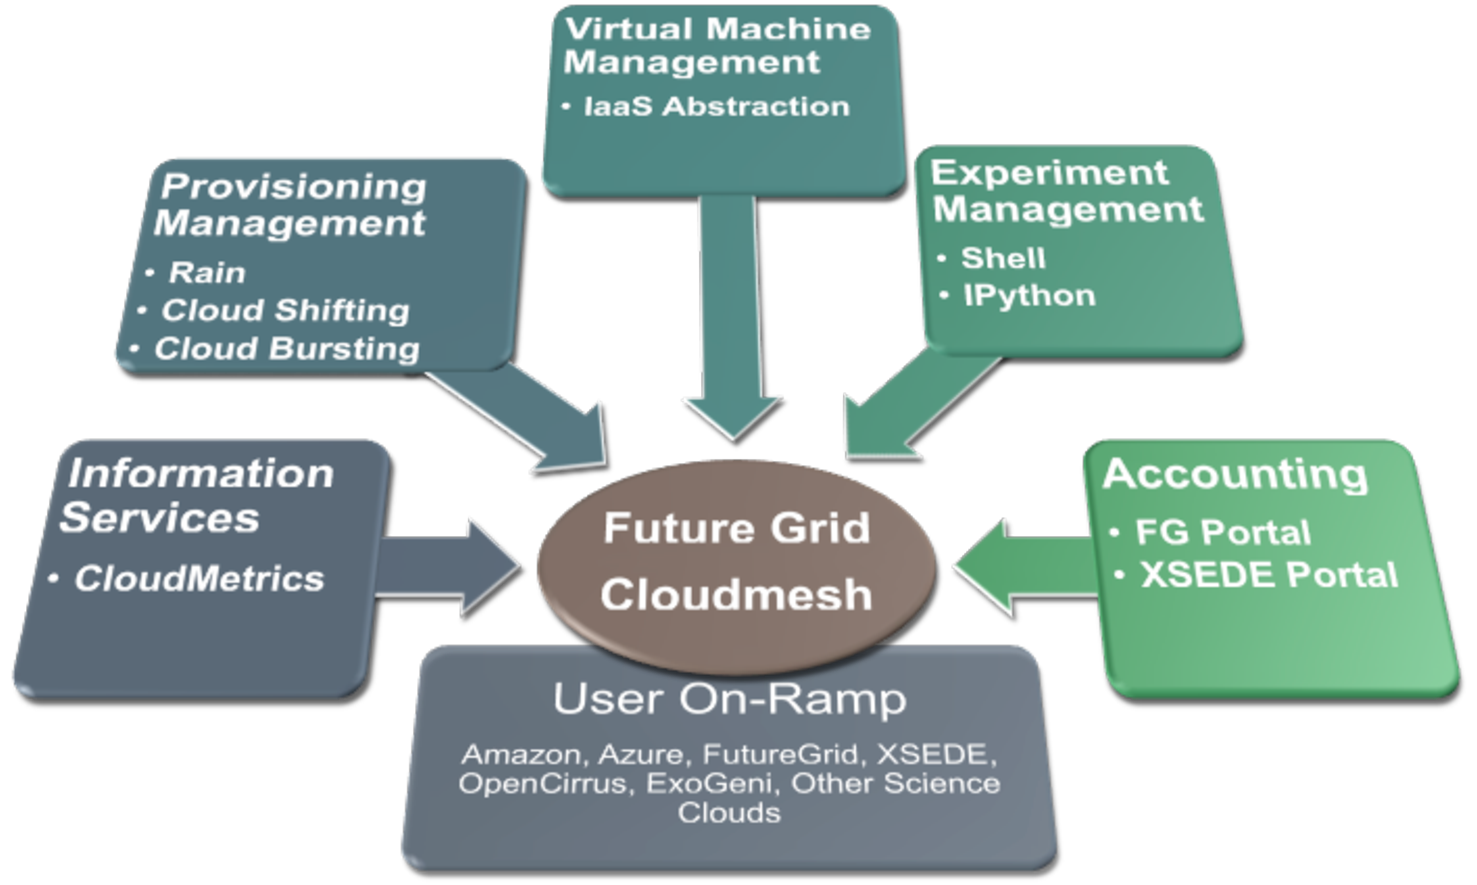
\includegraphics[width=1.0\columnwidth]{images/cm-functionality.pdf}
  \caption{CM Functionality.}\label{F:cm-func}
\end{figure}




\subsection{Architecture}


The three layers of the Cloudmesh architecture include a Cloudmesh Management Framework for monitoring and operations, user and project management, experiment planning and deployment of services needed by an experiment, provisioning and execution environments to be deployed on resources to (or interfaced with) enable experiment management, and resources.


\begin{figure}[htb]
  \centering
    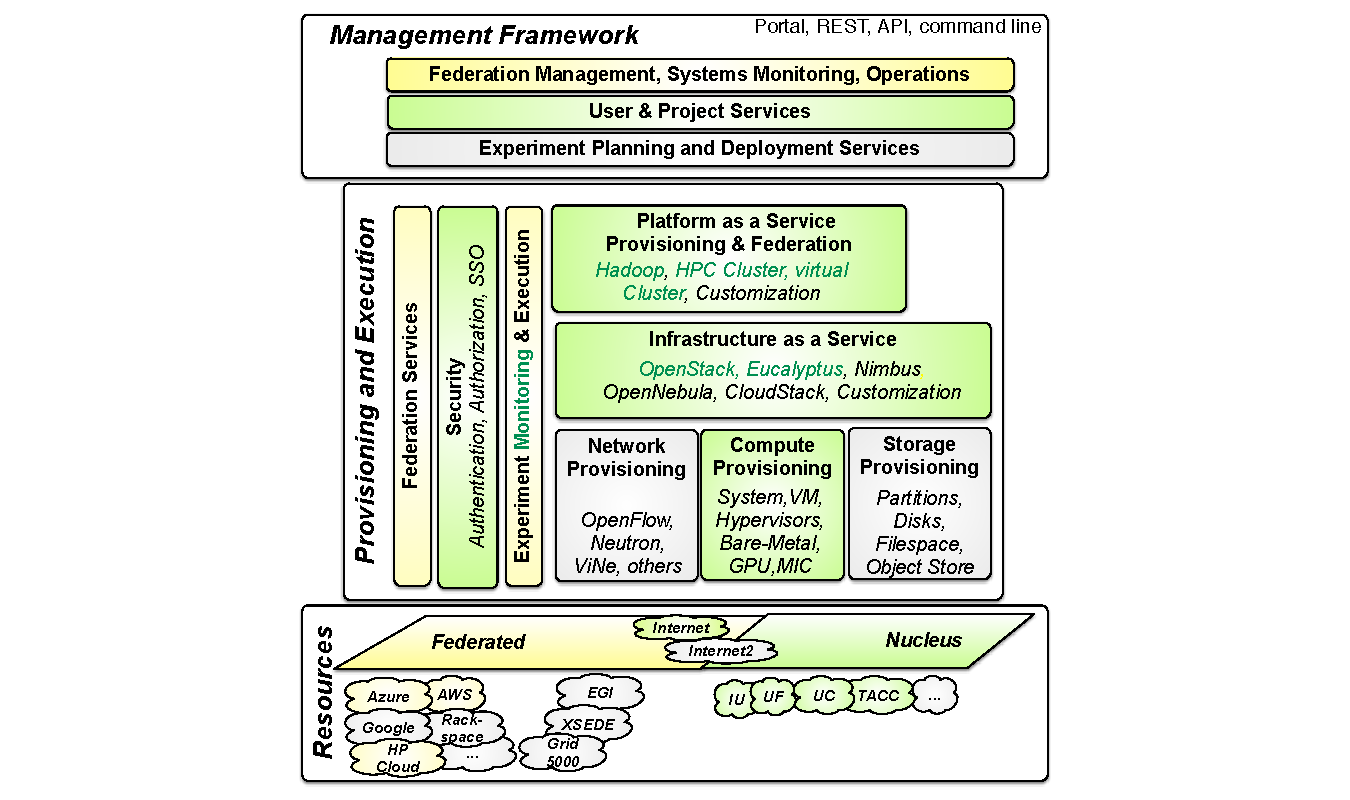
\includegraphics[width=1.0\columnwidth]{images/cm-arch.pdf}
  \caption{CM Architecture.}
\end{figure}


\paragraph{System Monitoring and Operations.}


The management framework contains services to facilitate FutureGrid day-to-day operation, including federated or selective monitoring of the infrastructure. Cloudmesh leverages FutureGrid for the operational services and allows administrators to view ongoing system status and experiments, as well as interact with users through ticket systems and messaging queues to inform subscribed users on the status of the system.
The Cloudmesh management framework offers services that simplify integration of resources in the FutureGrid nucleus or through federation. This includes, for user management, access to predefined setup templates for services in enabling resource and service provisioning as well as experiment execution. To integrate IaaS frameworks Cloudmesh offers two distinct services:


(a) a federated IaaS frameworks hosted on FutureGrid,
(b) the availability of a service that is hosted on FutureGrid, allowing the integration of IaaS frameworks through user credentials either registered by the users or automatically obtained from our distributed user directory.


For (b) several toolkits exist to create user-based federations, including our own abstraction level which supports interoperability via libcloud, but more importantly it supports directly the native OpenStack protocol and overcomes limitations of the EC2 protocol and the libcloud compatibility layer. Plugins that we currently develop will enable access to clouds via firewall penetration, abstraction layers for clouds with few public IP addresses and integration with new services such as OpenStack Heat. We successfully federated resources from Azure, AWS, the HP cloud, Karlsruhe Institute of Technology Cloud, and four FutureGrid clouds using various versions of OpenStack and Eucalyptus. The same will be done for OpenCirrus resources at GT and CMU through firewalls or proxy servers.
Additional management flexibility will be introduced through automatic cloud-bursting and shifting services. While cloud bursting will locate empty resources in other clouds, cloud shifting will identify unused services and resources, shut them down and provision them with services that are requested by the users. We have demonstrated this concept in 2012 moving resources for more than 100 users to services that were needed based on class schedules. A reservation system will be used to allow for reserved creation of such environments, along with improvements of automation of cloud-shifting.


\paragraph{User and Project Services}


FutureGrid user and project services simplify the application processes needed to obtain user accounts and projects. We have demonstrated in FutureGrid the ability to create accounts in a very short time, including vetting projects and users -- allowing fast turn-around times for the majority of FutureGrid projects with an initial startup allocation. Cloudmesh reuses this infrastructure and also allows users to manage proxy accounts to federate to other IaaS services to provide an easy interface to integrate them.


\paragraph{Accounting and App Store}


To lower the barrier of entry Cloudmesh will be providing a shopping cart which will allow checking out of predefined repeatable experiment templates. A cost is associated with an experiment making it possible to engage in careful planning and to save time by reusing previous experiments. Additionally, the Cloudmesh App Store may function as a clearing-house of images, image templates, services offered and provisioning templates. Users may package complex deployment descriptions in an easy parameter/form-based interface and other users may be able to replicate the specified setup with.
Due to our advanced Cloudmesh Metrics framework we are in the position to further develop an integrated accounting framework allowing a usage cost model for users and management to identify the real impact of an experiment on resources. This will be useful to avoid overprovisioning and inefficient resource usage. The cost model will be based not only on number of core hours used, but also the capabilities of the resource, the time, and special support it takes to set up the experiment. We will expand upon the metrics framework of FutureGrid that allows measuring of VM and HPC usage and associate this with cost models. Benchmarks will be used to normalize the charge models.


\paragraph{Networking}


in{ceWe have a broad vision of resource integration in FutureGridources be with systems offering different levels of control from bare metal to use of a portion of a resource. Likewise, we must utilize networks offering various levels of control, from standard IP connectivity to completely configurable SDNs as novel cloud architectures will almost certainly leverage NaaS and SDN alongside system software and middleware. FutureGrid resources will make use of SDN using OpenFlow whenever possible and the same level of networking control will not be available in every location.


\paragraph{Monitoring}


To serve the purposes of CISE researchers, Cloudmesh must be able to access empirical data about the properties and performance of the underlying infrastructure beyond what is available from commercial cloud environments. To accommodate this requirement we have developed a uniform access interface to virtual machine monitoring information available for OpenStack, Eucalyptus, and Nimbus. In the future, we will be enhancing the access to historical user information. Right now they are exposed through predefined reports that we create on a regular basis. To achieve this we will also leverage the ongoing work while using the AMPQ protocol. Furthermore, Cloudmesh will provide access to common monitoring infrastructure as provided by Ganglia, Nagios, Inca, perfSonar, PAPI and others.

\subsection{Cloud Shifting}


We have already demonstrated via the RAIN tool in Cloudmesh that it is possible to easily shift resources between services. We are currently expanding upon this idea and developing more easy to use user interfaces that assist administrators and users through role and project based authentication to move resources from one service to another (see Figure \ref{F:shift}).


\begin{figure}[htb]
  \centering
    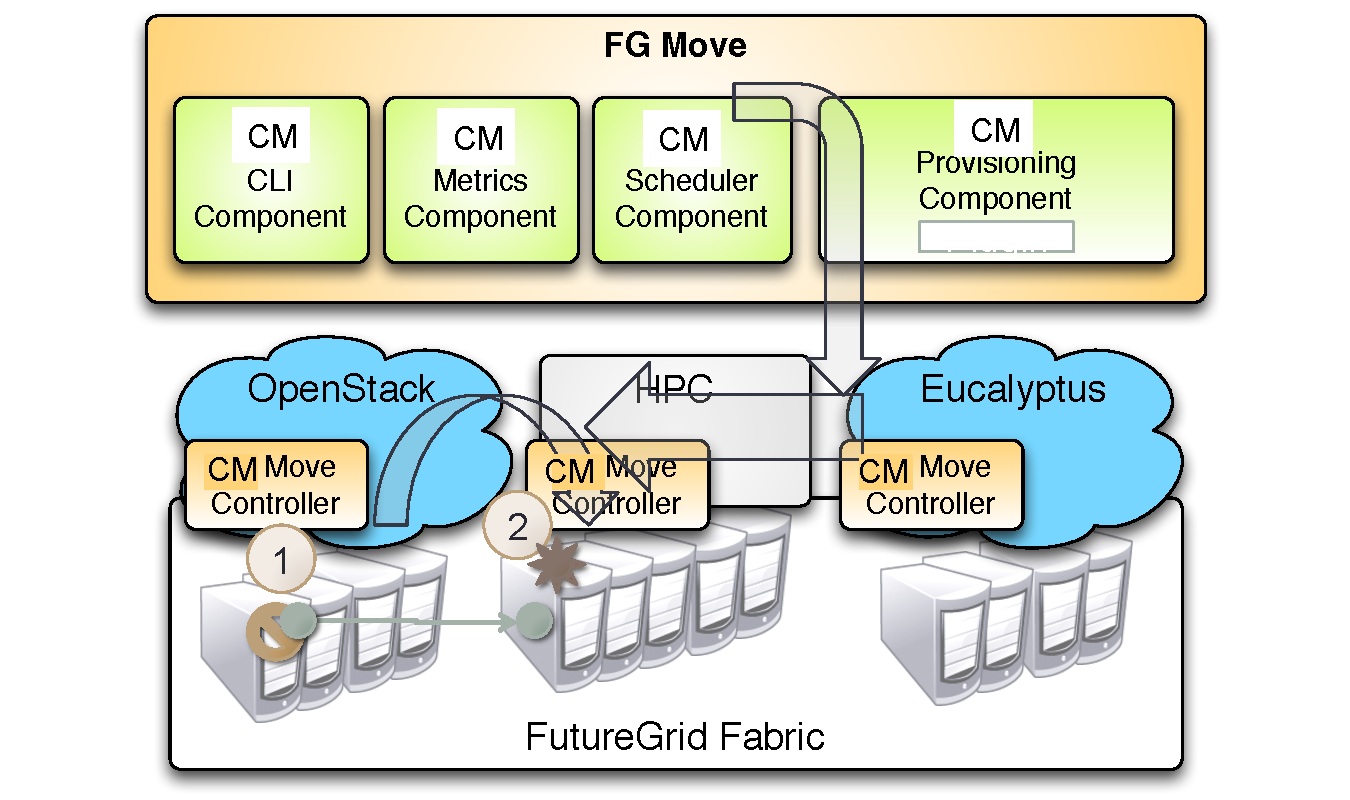
\includegraphics[width=1.0\columnwidth]{images/shift2.pdf}
  \caption{Shifting resources makes it possible to offer flexibility
    in the service distribution in case of over or underprovisioning.}\label{F:shift}
\end{figure}
v

\subsection{Graphical User Interface}


Despite the fact that Cloudmesh was originally a quite sophisticated command shell and command line tool, we have spend recently more time in exposing this functionality through a convenient Web interface. Some more popular views if this interface are depicted in Figure \ref{F:instances} hinting on how easy it is with a single button to create multiple VMs across a variety of IaaS. Also nice is that this not only includes resources at IU but also at external locations. Pushing this easy management in a more sophisticated experience for the user while associating one-click deployments that include the ability to deploy virtual clusters, Hadoop environments, and other more elaborate setups we provide an early prototype screenshot in Figure \ref{F:oneclick}.


\begin{figure}[htb]
  \centering
    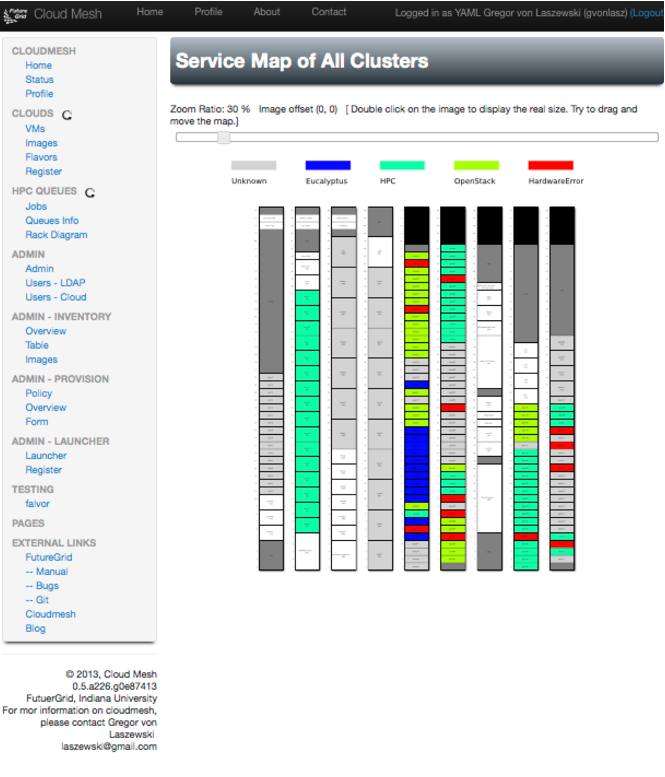
\includegraphics[width=1.0\columnwidth]{images/rainbow.pdf}
  \caption{Monitoring the Service distribution of FutureGrid with Cloudmesh.}
\end{figure}


\begin{figure}[htb]
  \centering
    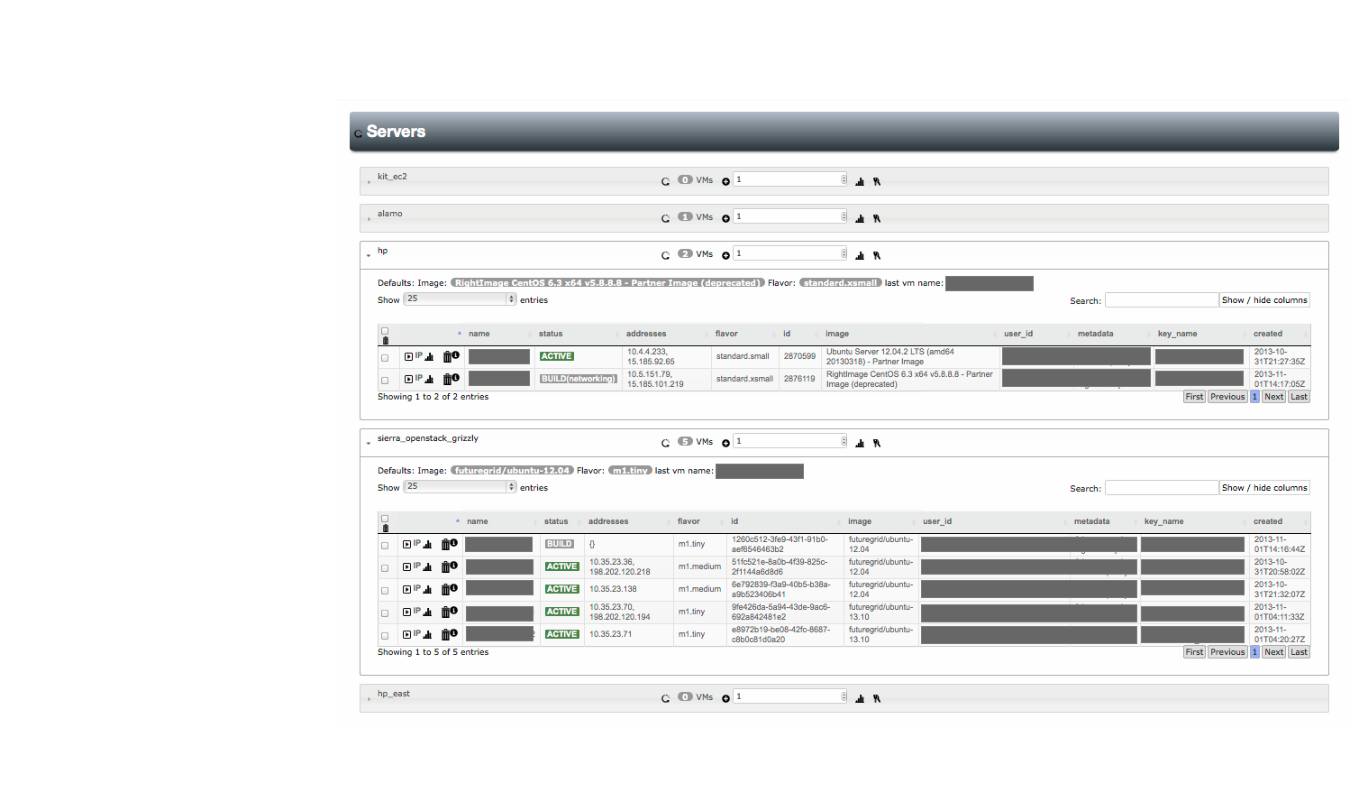
\includegraphics[width=1.0\columnwidth]{images/instances.pdf}
  \caption{Screenshot demonstrating how easy ot is to manage multible VMs accross various clouds.}\label{F:instances}
  \centering
    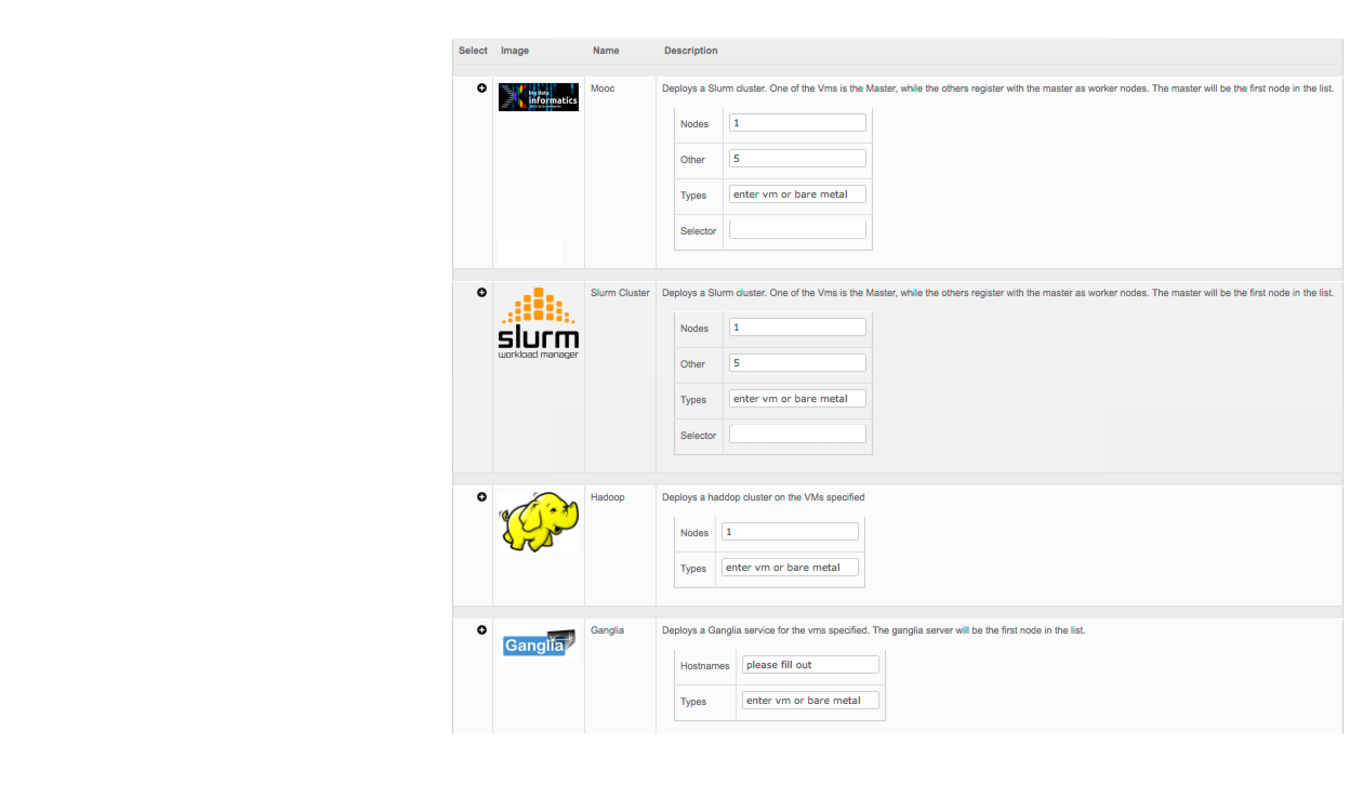
\includegraphics[width=1.0\columnwidth]{images/oneclick.pdf}
  \caption{One click deployment of platforms and sophisticated
    services that could even spawn multiple resources.}\label{F:oneclick}
\end{figure}

\section{Cloud Metrics}

Based on lessons learned from FutureGrid, knowledge of the resource
allocation an utilization is important to provide users and
administrators with a holistic infrastructure picture in order to guide
utilization according to set goals.

This is especially of interest as FutureGrid supports more than 380
projects and 2300 users are supported and resource cloud become over
provisioned or are not properly used by the users. Among the many
services that FutureGrid offers we have especially focussed on those
that are highly used including OpenStack, Eucalyptus, Nimbus, and
batch systems supported by Moab and Torque.  These services are
partially installed on several distributed clusters.

For this paper we will restrict our discussion on the IaaS based
monitoring components. As the systems did not provide any sufficient
monitoring capabilities, and if they existed they were not unified, we
have developed a federated CloudMesh Metrics system that aggregates
the information from distributed clusters and a variety of
heterogeneous IaaS services, such as OpenStack, Eucalyptus, and
Nimbus. Other HPC related activities in regards to monitoring and
metrics are discussed in \cite{ubmod}
and \cite{las12xdmod-kernel,las12xdmod-planing,las13xdmod}.


The two main components of CloudMesh Metrics (a) measure the resource
allocation across several IaaS platforms and (b) provide statistics
and usage data through various user interface while at the same time
servicing distinct user communities. This includes the user that is
interested in monitoring his own utilization, the project that may
constitute multiple users, and the service provider that is interested
in offering optimized services to the users and projects.

\subsection{User- and Project-based Metrics Services}

In order for users to use a variety of clouds it is important for them
to monitor and compare their resource utilization on the various
clouds. It is important to note that this may not only mean for
individual users, but also for users that are organized as part of a
joint project. Users can naturally be in multiple projects, or have
access to multiple clouds. Thus the requirement exists to present the
data to the user based on individual user utilization, group,
utilization, or even experiment utilization, where a particular
experiment is analyzed instead of just looking at the total
utilization.

\subsection{Resource Provider-based Metrics Services}

In addition to providing a great deal of information about each user,
a holistic metric system that enables an overview of the various
resource metrics is important for resource providers. It is clear that
summary information may be customized based on the requirements by
individual users, project leads, resource providers, site managers,
and funding agencies. This information is typically restricted to the
actual {\em resources} for which administrative access exists in order
to provide a holistic set of metrics.
To enable this holistic view we will first start by basing our inotial
development efforts on the extension of the CLoud Metrics services
that have been developed by FutureGrid for a multi-cloud environment
for resource providers within FutureGrid.
The extensions will include that ability to alos integrate public and other cloud
information offered as part of the multi-cloud infrastructure
accessible to the users today.

\subsection{CloudMesh Metric Architecture}

The cloudmesh metric architecture is based on the integration of a
authorized REST service, that utilizes a simple abstraction layer to interface
with the various cloud services to obtain needed information gathered
under authorization constraints. The data will be hosted in a NOSQL
database to allow mining of the data in map/reduce frameworks. Data
can be ingested either directly through the database via the API, or
through REST calls that are mitigated through message queues with
AMPQ. Adapters can be written to integrate new information providers 


\begin{figure}[htb]
  \centering
    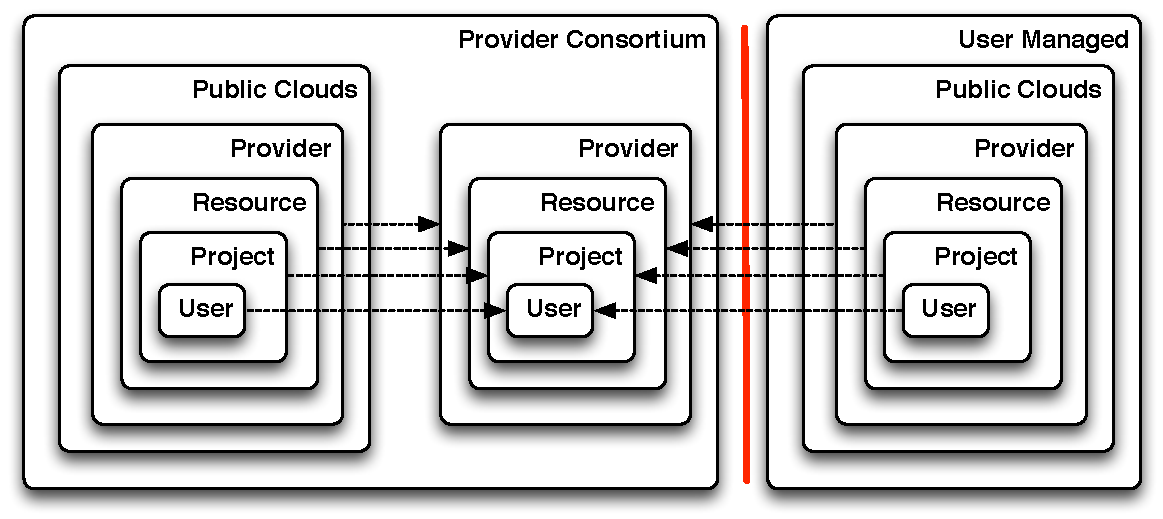
\includegraphics[width=1.0\columnwidth]{images/metric-hierarchy.pdf}
  \caption{Integration Hierarchy to access cloud metrics as part of 
    provider and user managed multi-clouds.}
  \label{F:metric-arch}
\end{figure}


compare to: \cite{smith13info}

\subsection{CloudMesh Metrics: Measuring Resource Utilization}

%\begin{figure}[htb]
%  \centering
%    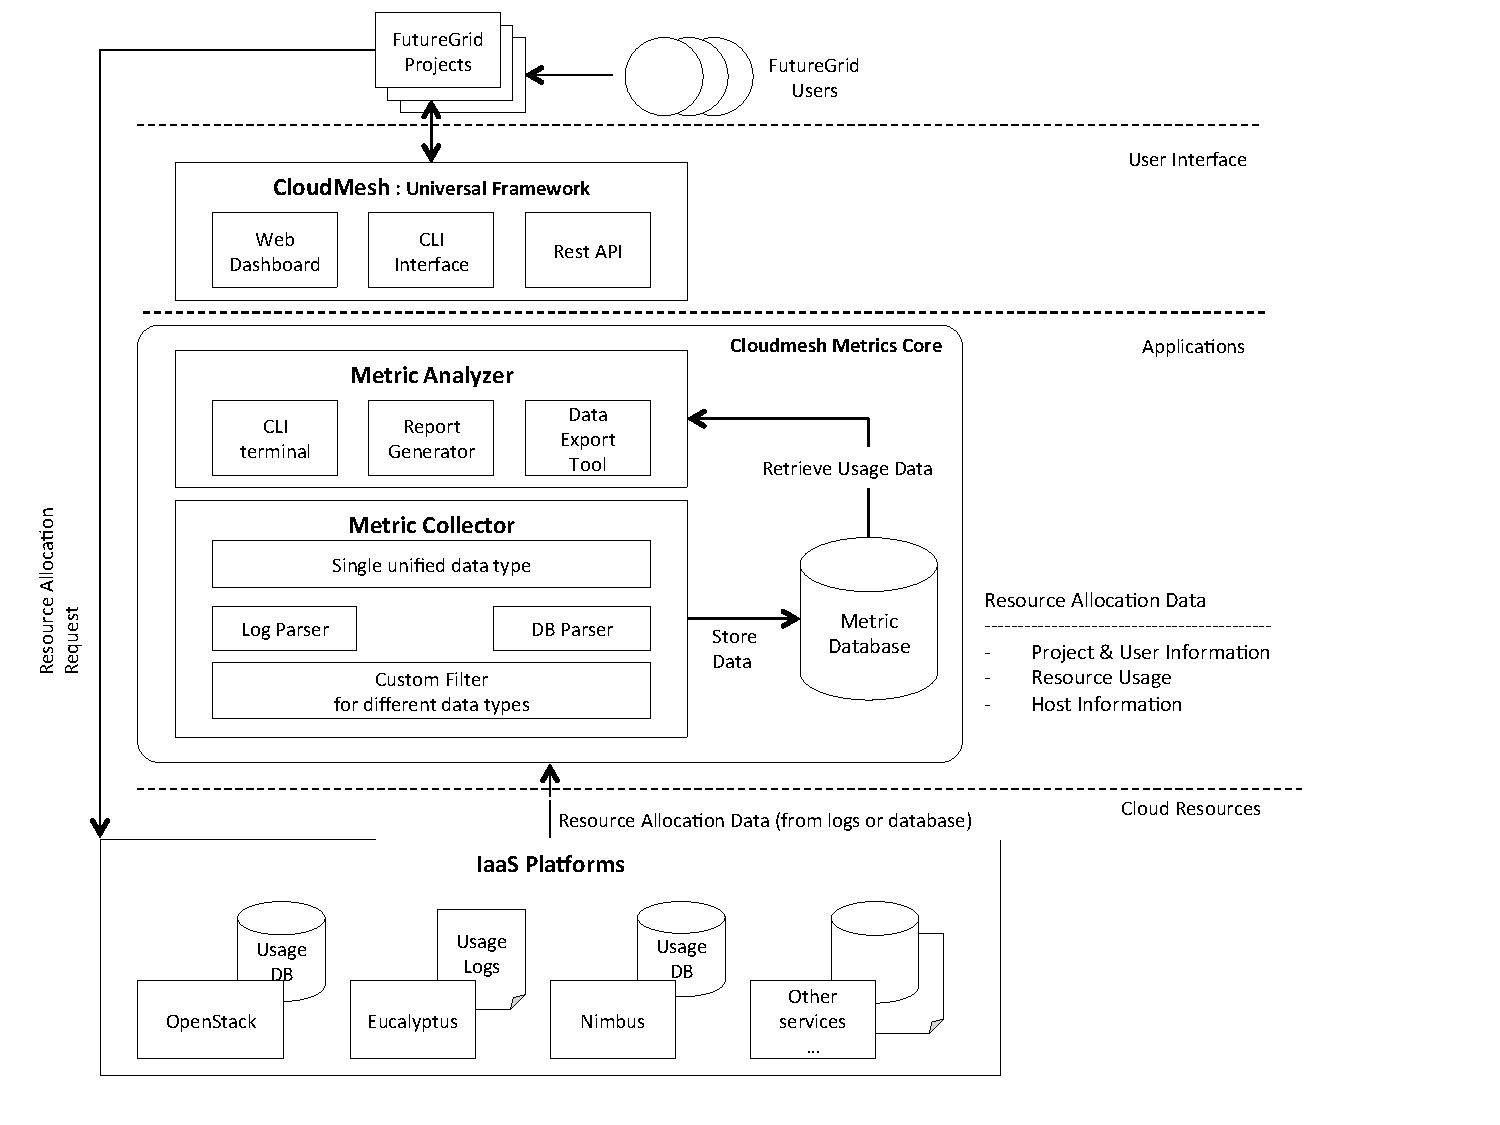
\includegraphics[width=1.0\columnwidth]{images/cloudmesh-metrics.pdf}
%  \caption{Design of CloudMesh Metrics Architecture}
%  \label{F:metric-arch}
%\end{figure}
 
The current Cloudmesh MetricCollector offers OpenStack, Eucalyptus, and Nimbus but not
limited to these platforms. The pre-defined filters help collect usage
data from any cloud platforms and data resource (e.g. log files,
mysql, or sqlite). Representing measured data is one of the key roles
in CloudMesh Metrics to help understand the data. It is often to
happen to interpret data improperly which may result in an incorrect
conclusion. With visualization tools and Command-Line Interface
provided by Cloud Analyzer, the chances of misuse of statistics can be
diminished. External visualization toolkits and exporting tools have
been used to describe usage information without unnecessary
interpretation. The measured data by Metrics is represented in
CloudMesh which is a universal framework of managing any compute
resources. CloudMesh consists of several components that manage
accounts and handle compute resources not only in FutureGrid, but also
in any other compute resources. With the Rest API, the metrics data
can be presented by CloudMesh.

 



\subsection{Metric Collector}

The process of measuring resource allocation begins with collecting
usage data within the infrastructure. Each IaaS cloud resource
provider typically has an internal system to record resource
allocation per users or groups. Virtual Instance is a good measure of
resource utilization in cloud environments since it reserves and
releases compute resource when it deploys. To measure the amount of
resources allocated and consumed, CloudMesh Metrics places the Metric
Collector to IaaS platforms. For example, the metric collector
periodically connects to OpenStack database to obtain information of
VM deployment. Once the collecting process has been completed,
unifying different data types of the measured data is critical to
provide a summary of resource allocation across several IaaS
platforms. The filter of the metric collector converts the data types
into a single data object consisting of attribute-value pairs in
Metrics database.To achieve this goal, NoSQL database is recommended
in the metrics system.  Table~\ref{T:compare-iaas} shows details of
measuring resource allocation on FutureGrid.

\subsection{Metric Analyzer}

The purpose of the Metric Analyzer in CloudMesh is to provide ways for
processing statistics and interacting with users to get the proper
interpretation of data. Visualization of measured data is offered to
ease understanding of the data using chart
tools. ~\cite{kosslyn1989understanding,pinker1990theory,friel2001making}. Metric
Analyzer suggests three components to accomplish these goals. CLI
terminal provides an interactive shell so that users can specify
details of getting statistics e.g. region, cluster, user, project
names, etc. With the python cmd module, it is easy to build custom
commands that directly retrieve the usage data. Available metrics and
commands are listed with the built-in help commands that are generated
by automatic docstring translation. If a formal representation of data
is preferred with graphical chart tools, Report Generator in CloudMesh
Metrics can be used to provide web-based reports with different type
of charts, e.g. histogram, bar chart, pie chart or line chart. Report
Generator publishes documentation in HTML and PDF formats using python
Sphinx system~\cite{brandl2009sphinx}, external chart tools
i.e. highcharts ~\cite{highsoft2012highcharts} and Google Chart API,
etc. The metrics with different chart types in table \~ref{Table:2}
are included in the documentation generated by Report
Generator. Referencing data can be simply done via downloading a csv
or json format file in Data Export Tool.




Note:
Table \ref{T:compare-iaas}

    Nimbus: create\_event, remove\_event tables 
    OpenStack: nova, keystone  databases 

    Eucalyptus: cc.log, Compute Log 


%\newcommand{\YES}{\checkmark}
%\newcommand{\NO}{\textopenbullet}
\newcommand{\YES}{\ding{51}}

\newcommand{\NO}{\ding{55}}


\begin{table}[h!]
  \caption{Measurement of IaaS on FutureGrid}\label{T:compare-iaas}
  ~\\
  \begin{small}
  \begin{tabularx}{\columnwidth}{|l|X|X|X|}
  \hline
                 & {\bf Nimbus} & {\bf OpenStack} & {\bf Eucalyptus} \\
    \hline
    \hline
    \multicolumn{4}{|l|}{\bf Documentation of the Data Sources} \\
    \hline
       & \NO & \YES & \YES \\
    \hline
    \hline
    \multicolumn{4}{|l|}{\bf Data Sources} \\
    \hline
         & sqlite3 & MySQL & Log Files \\
    \hline
    \hline
    \multicolumn{4}{|l|}{\bf Metrics} \\
    \hline
    ~~vCPU core & \YES & \YES & \YES \\
    ~~memory & \YES & \YES & \YES \\
    ~~disk & \YES & \YES & \YES \\
    ~~instance type   & \NO & \YES & \YES \\
    ~~host & \YES & \YES & \YES \\
    \hline
    \hline
    \multicolumn{4}{|l|}{\bf Account Management Features} \\
    \hline
    ~~Users     & \YES & \YES & \YES \\
    ~~Projects & \NO & \YES & \YES \\
    \hline
    \hline
    \multicolumn{4}{|l|}{\bf Cluster} \\
    \hline
    ~~Alamo  & \YES & \YES & \NO \\
    ~~Foxtrot & \YES & \NO & \NO \\
    ~~Hotel    & \YES & \YES & \NO \\
    ~~India     & \NO  & \YES & \YES \\
    ~~Sierra    & \NO & \YES & \YES \\
    ~~Lima     & ?       &  ?      &  ?       \\   
    \hline
%    Region& \shortstack[l]{TACC$^1$, \\UF$^2$, \\UChicago$^3$, \\SDSC$^4$} & \shortstack[l]{TACC, \\IU$^5$, \\SDSC } & \shortstack[l]{IU, \\SDSC$^6$} \\
%    \hline
  \end{tabularx}\\
%  $^1$ Texas Advanced Computing Center \\
%  $^2$ University of Florida \\
%  $^3$ University of Chicago \\
%  $^4$ San Diego Supercomputing Center\\
%  $^5$ Indiana University\\
%  $^6$ in early 2014\\
\end{small}
\end{table}

\subsection{Metric Analyzer}

The purpose of the Metric Analyzer in CloudMesh is to provide ways for processing statistics and interacting with users to get the proper interpretation of data. Visualization of measured data is offered to ease understanding of the data using chart tools. ~\cite{kosslyn1989understanding,pinker1990theory,friel2001making}. Metric Analyzer suggests three components to accomplish these goals. CLI terminal provides an interactive shell so that users can specify details of getting statistics e.g. region, cluster, user, project names, etc. With the python cmd module, it is easy to build custom commands that directly retrieve the usage data. Available metrics and commands are listed with the built-in help commands that are generated by automatic docstring translation. If a formal representation of data is preferred with graphical chart tools, Report Generator in Metric Analyzer can be used to provide web-based reports with different type of charts, e.g. histogram, bar chart, pie chart or line chart. Report Generator publishes documentation in HTML and PDF formats using python Sphinx system~\cite{brandl2009sphinx}, external chart tools i.e. highcharts ~\cite{highsoft2012highcharts} and Google Chart API. The metrics with different chart types in Table~\ref{T:iaas-with-graph} are included in the documentation generated by Report Generator. Referencing data can be simply done via downloading a csv or json format file in Data Export Tool. With these tools, such as cli terminal, sphinx report generator, and exporting tool, CloudMesh users have access to the metrics in various ways.


\begin{table}[h!]
  \caption{Metric visualization with graphs}\label{T:iaas-with-graph}
  ~\\
  \begin{center}
  \begin{small}
  \begin{tabular}{|p{0.2\columnwidth}|p{0.7\columnwidth}|}
  \hline
  {\bf Example} & {\bf Description} \\
    \hline
    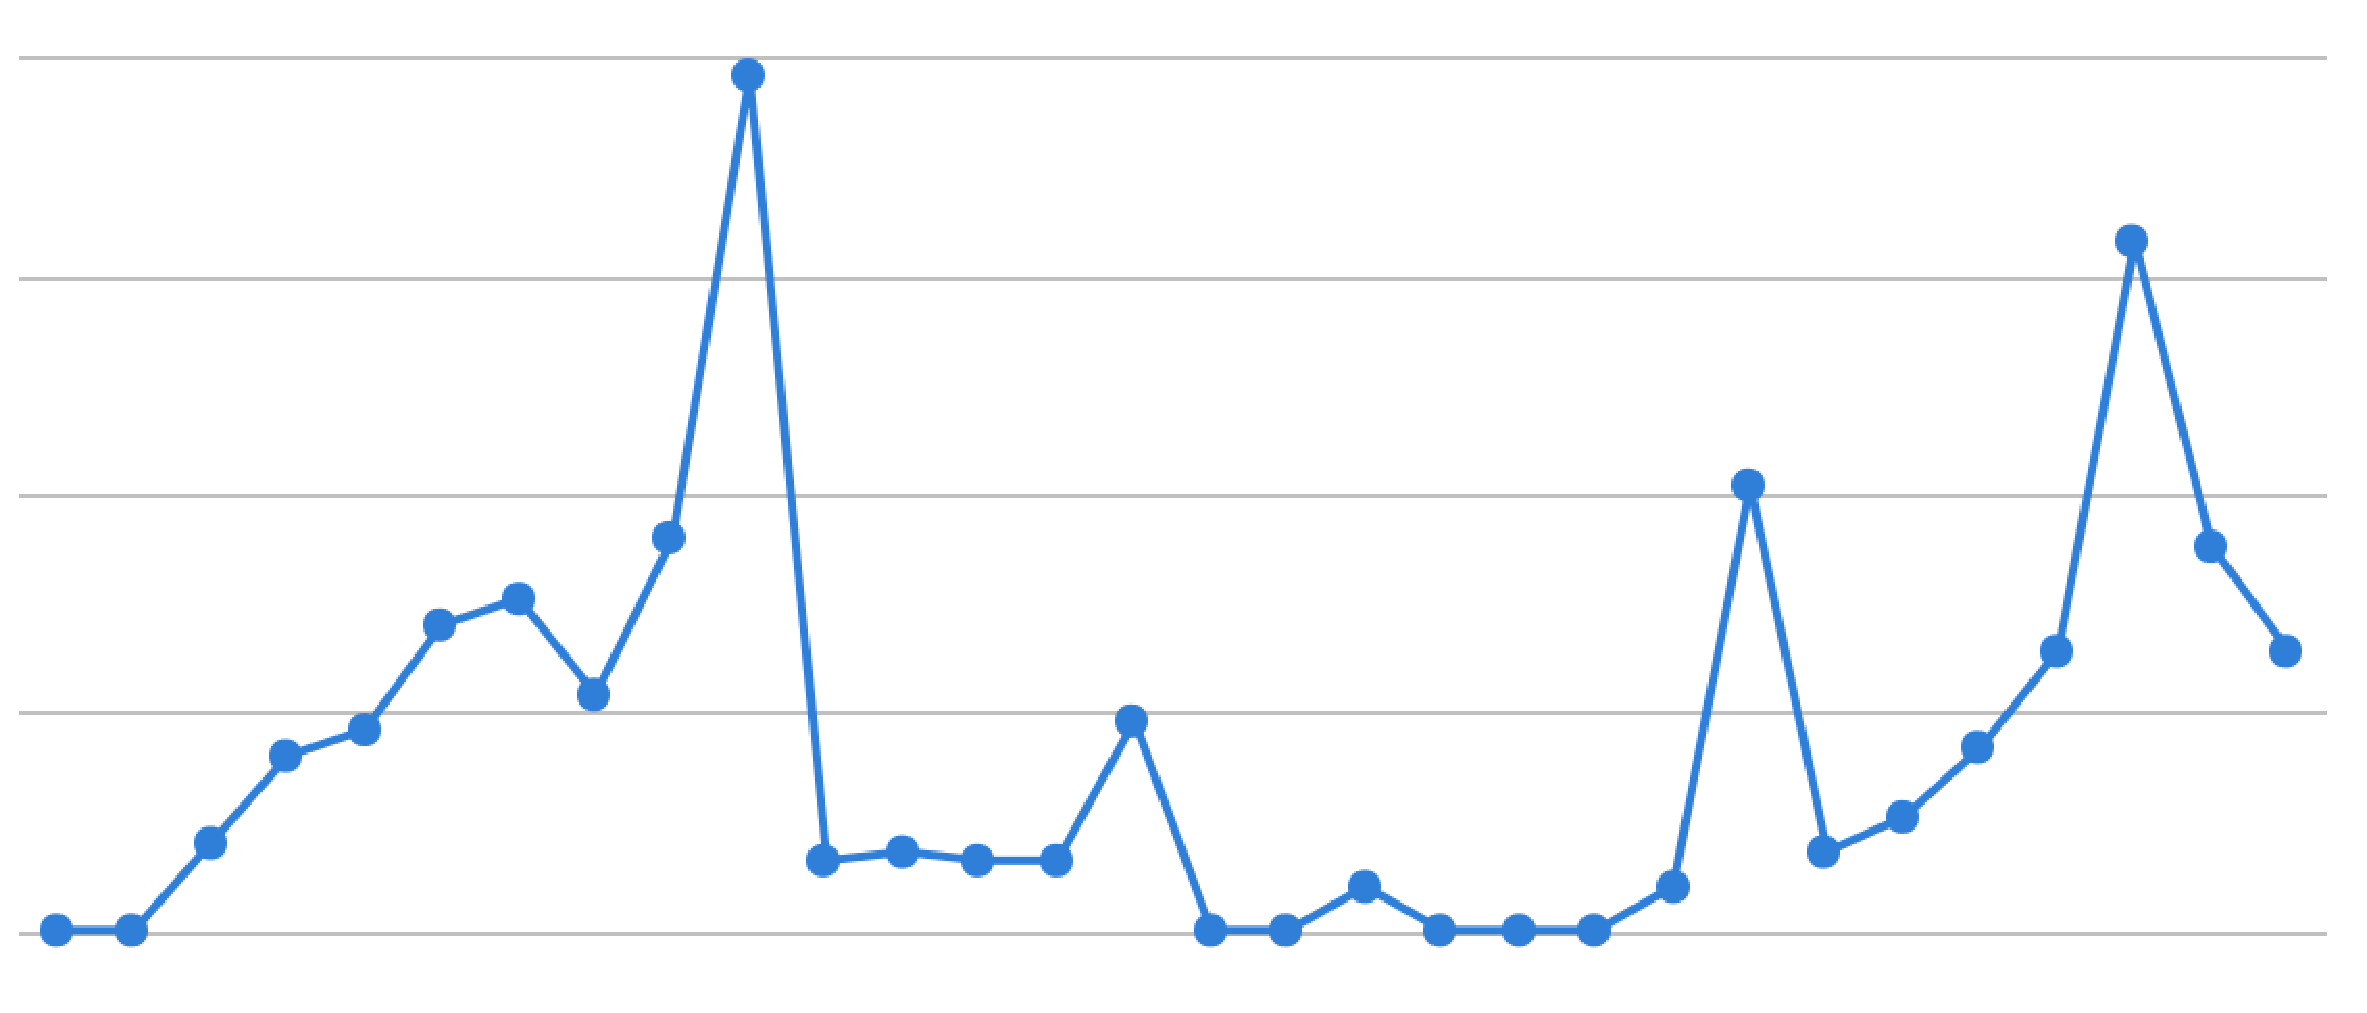
\includegraphics[width=0.2\columnwidth]{images/metric-line-chart.pdf} &  vCPU, Memories, Disks, and user count \\
    \hline
    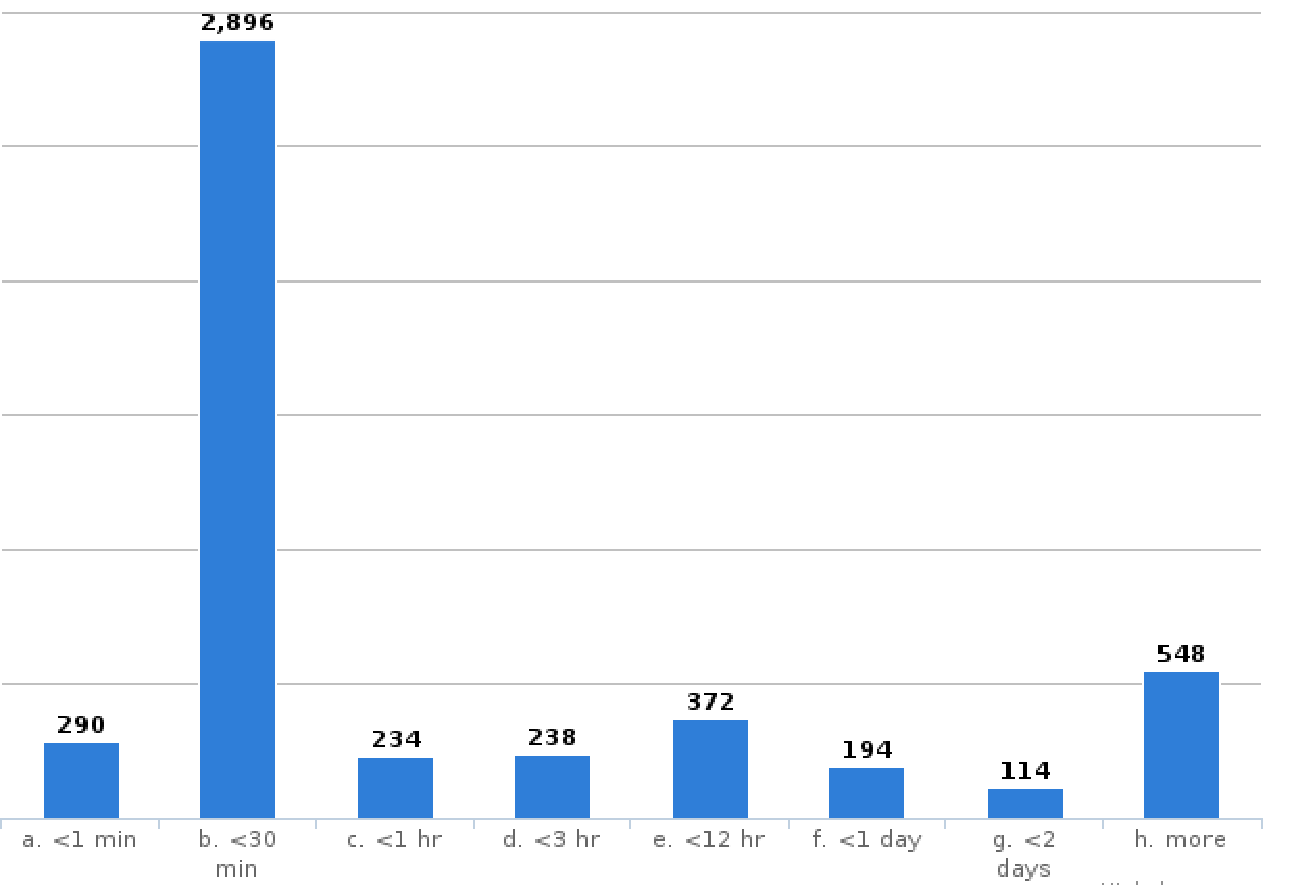
\includegraphics[width=0.2\columnwidth]{images/metric-histogram-chart.pdf} & Instance types \\
    \hline
    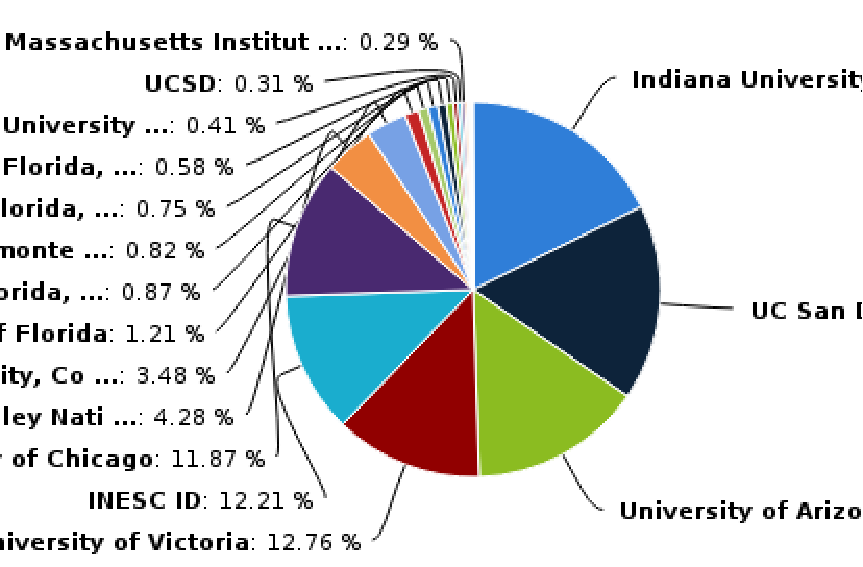
\includegraphics[width=0.2\columnwidth]{images/metric-pie-chart.pdf} & Regions, hosts \\
    \hline
    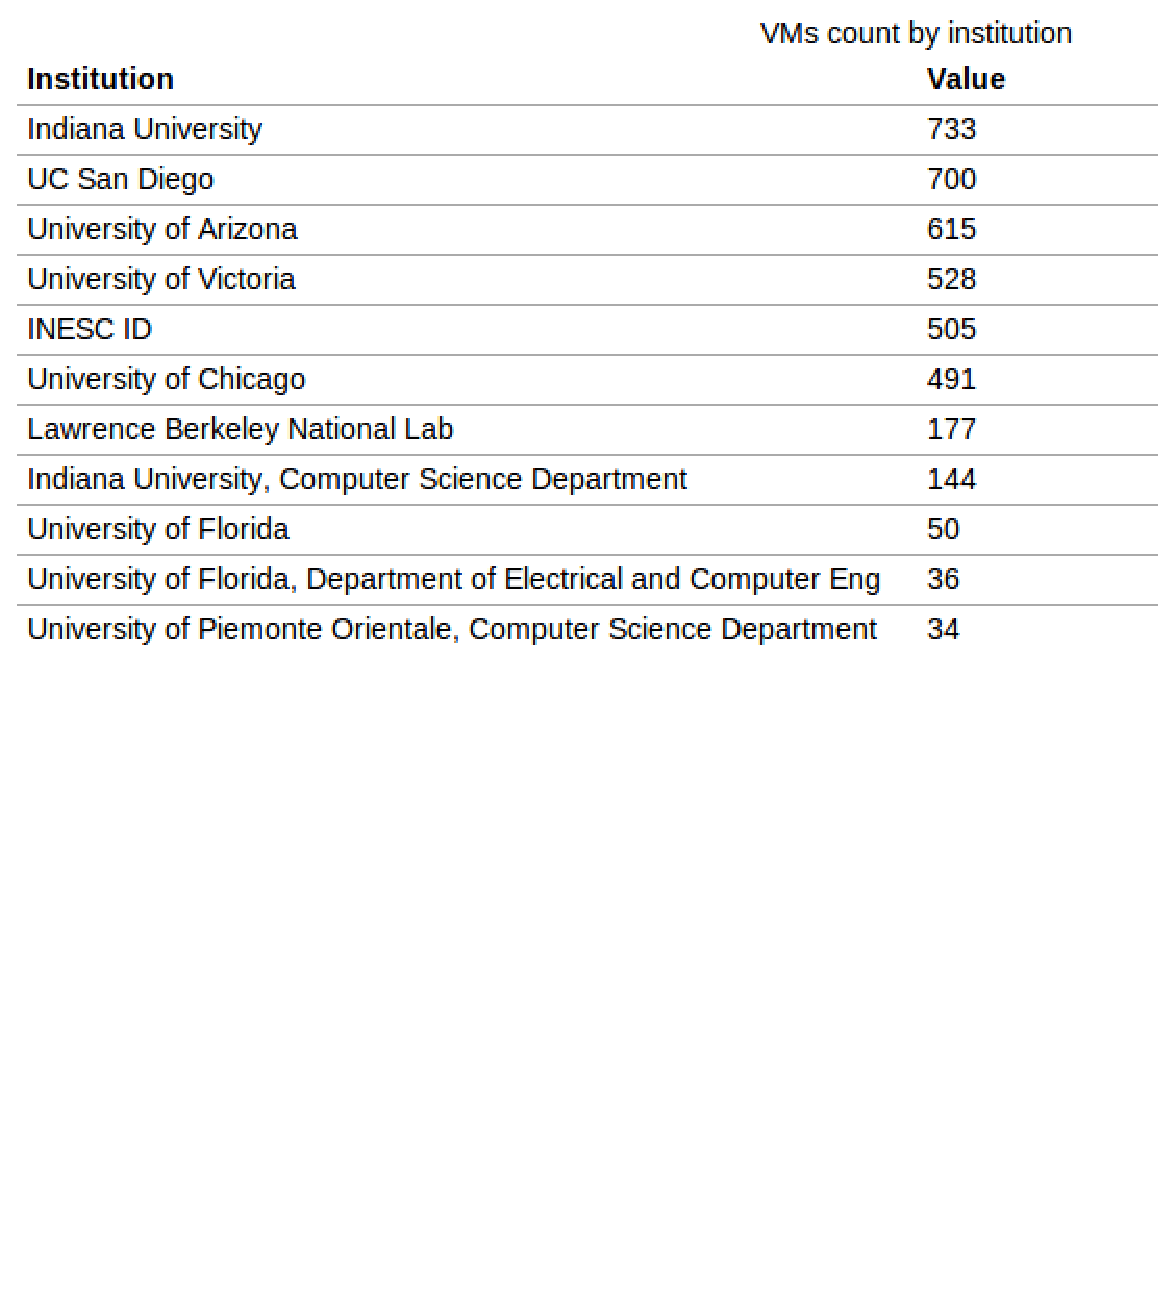
\includegraphics[width=0.2\columnwidth]{images/metric-table-chart.pdf} & Project leaders \\
    \hline
  \end{tabular}\\
\end{small}
\end{center}
\end{table}


%\clearpage 
 
%\bibliographystyle{IEEEtranS}
\bibliographystyle{IEEEtran}
%\bibliographystyle{abbrv} 
\bibliography{% 
bib/vonLaszewski-jabref.bib,%
bib/cyberaide-cloud,%
bib/cyberaide-metric} 
 
\end{document} 






